% Chapter Template

\label{chpt:observations and observational techniques} % for referencing this chapter elsewhere, use \ref{chpt:label}
\lhead{\emph{Observations, and observational techniques}} % This is for the header on each page - perhaps a shortened title

For CVs with a sufficiently high inclination ($\gtrsim 80 \deg$, depending on mass ratio) the donor will eclipse all other components of the system in quick succession, once per orbit. Observing and modelling these eclipses, with knowledge of the orbital period and the temperature of the white dwarf, can yield a thorough characterisation of the CV. The methodology for this characterisation is described in detail in \S\ref{chpt:modelling and techniques}, but essentially relies on extracting the white dwarf temperature and radius from the white dwarf colours and system parallax, and combining the white dwarf radius with the timing of eclipse features to find the component masses, donor radius, and orbital separation. Hence, to properly characterise a CV, we need flux-calibrated, high time resolution, multi-colour photometery of the target. 

The work of this thesis has made extensive use of three instruments: ULTRASPEC, ULTRACAM, and HiPERCAM.
These are time-series photometric imaging cameras, capable of taking high-cadence images of the night sky in one, three, or five colours, respectively. Crucially, HiPERCAM and ULTRACAM make their multi-colour images simultaneously, which removes the possibility of changes in brightness in the disc or bright spot polluting the white dwarf colour measurement. The eclipses we observe typically span around 30 minutes and need to measure flux changes on timescales of a few seconds to be useful for analysis, and these three cameras are ideal for this task.


\section{Instruments}

The cameras used were mounted on several telescopes across the decade of our observations. These were the Gran Telescopio de Canarias (GTC) on La Palma (with HiPERCAM), the Thai National Telescope (TNT) with ULTRASPEC, the New Technology Telescope (NTT) in Chil\'e (with ULTRACAM). Prior to \todo{When was ULTRACAM taken off the WHT? 2014, I think?}, ULTRACAM was hosted on the William Herschel Telescope (WHT), also on La Palma. 


\subsection{HiPERCAM}

HiPERCAM is an impressive quintuple-beam optical imaging camera that saw first light on the GTC in 2018, and is sensitive to wavelengths between $320 - 1060 \rm nm$ \citep{dhillon2021}. 
This camera has a series of dichroic beamsplitters, that sequentially pick off the $u_s, g_s, r_s, i_s, z_s$ bands and funnel each into dedicated cameras that use highly sensitive, low readout noise electron-multiplying CCDs. 
These Super SDSS filters are specifically designed for HiPERCAM to match the classic SDSS band cutoff wavelengths \citep{fukugita1996}, but allow a higher throughput and so give a more sensitive instrument. 
However, this improvement is not constant across the bands, shown in Figure~\ref{fig:observations:superSDSS throughput comparison}, resulting in a small difference between colours observed with HiPERCAM and SDSS. 
Unfortunately, as our calibrating standard stars are reported in the classic SDSS photometric system, some work was necessary to color-correct the HiPERCAM observations, which is described in detail in \S\ref{sect:observations:colour correction method}.
\begin{figure}
    \centering
    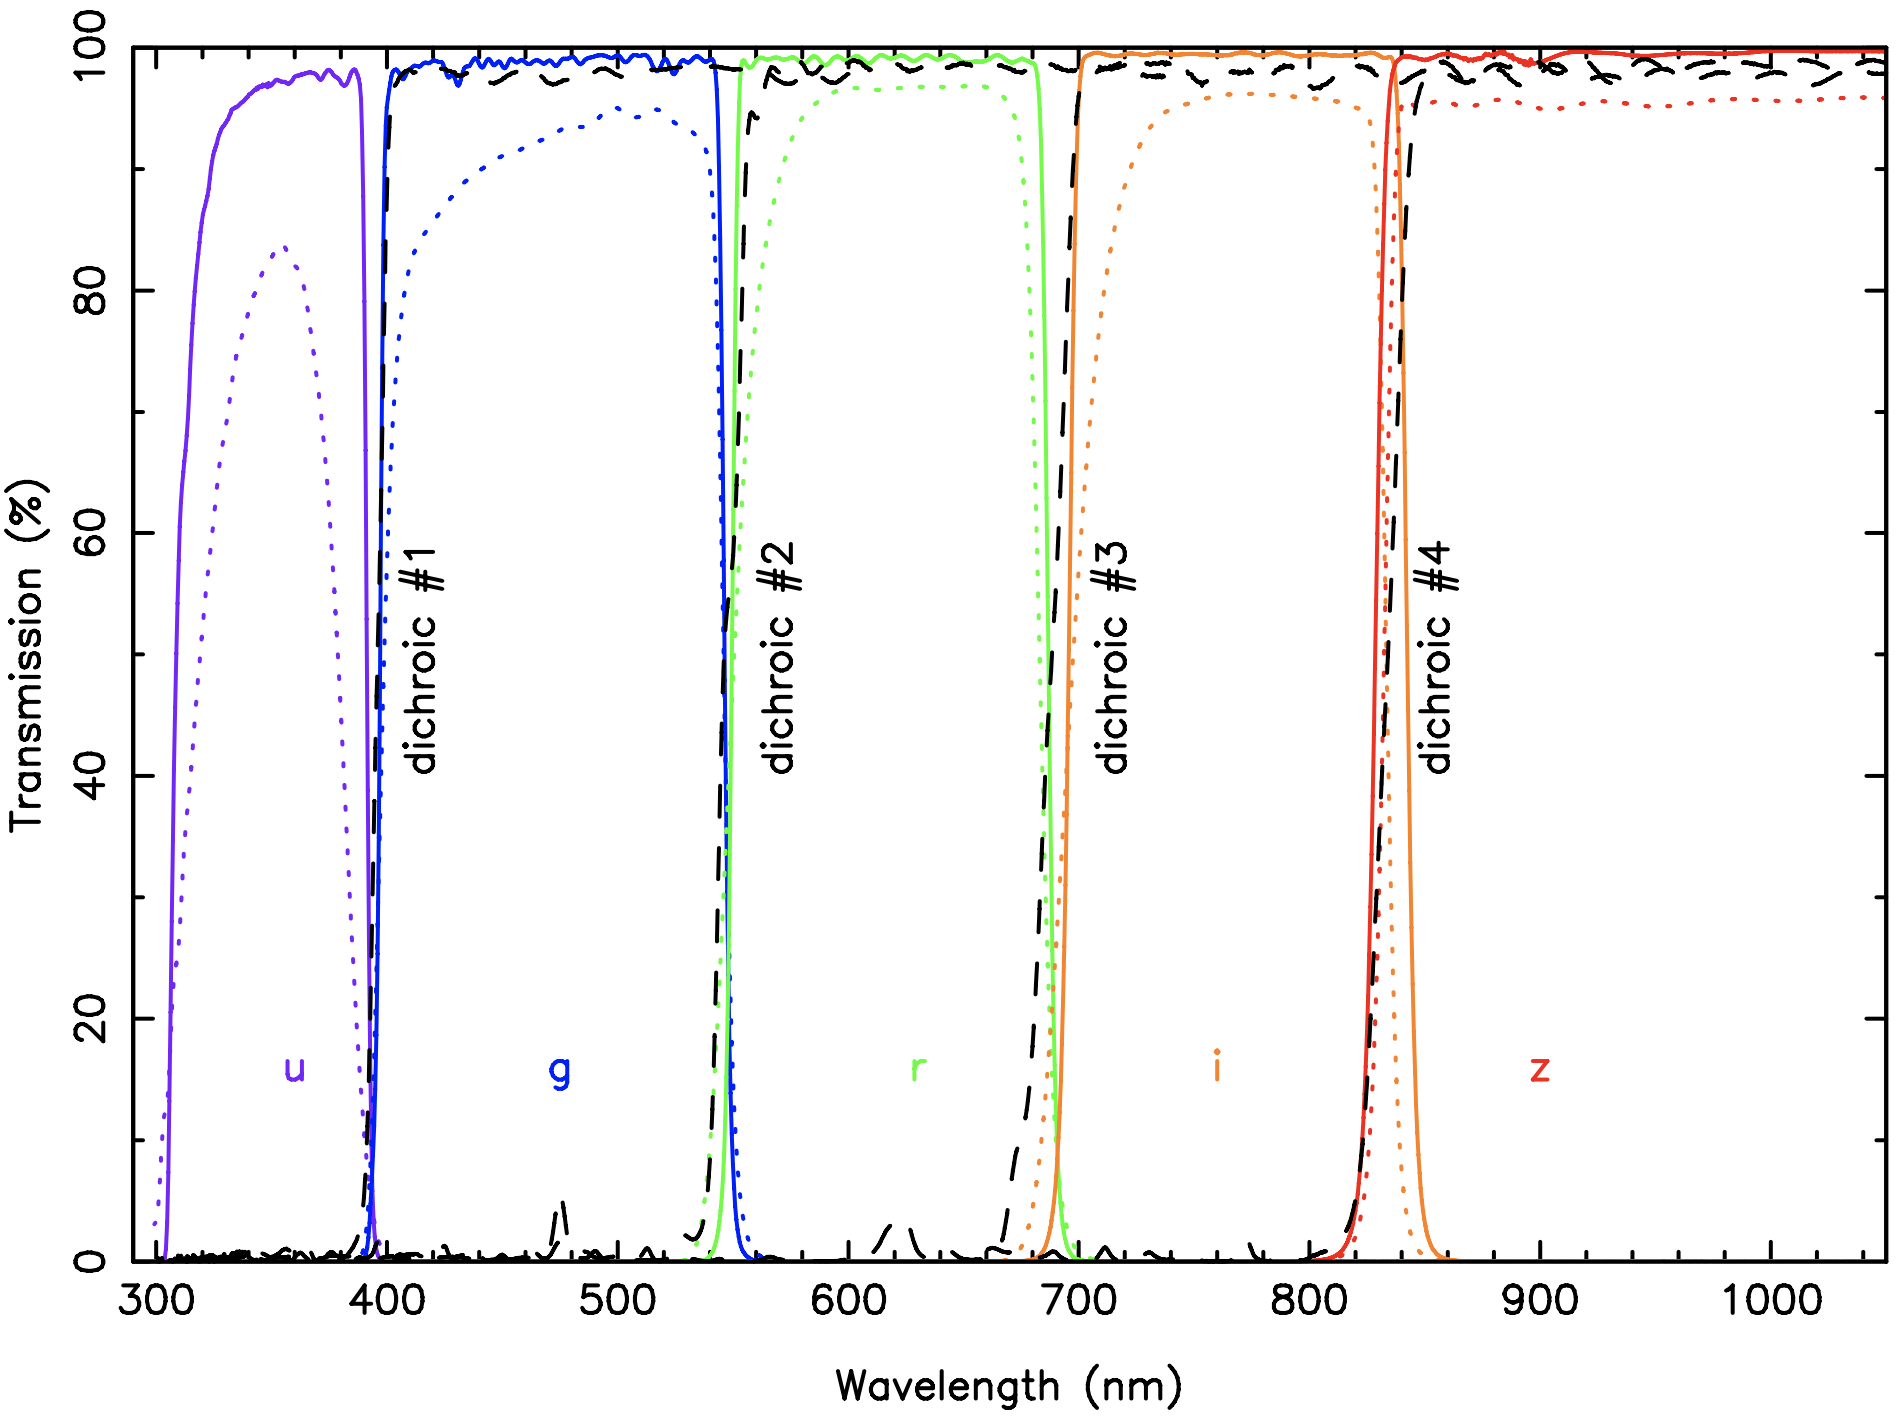
\includegraphics[width=0.7\textwidth]{figures/observations/plot_dichs_supersdss_asbuilt_v3.png}
    \caption{Taken from \citet{dhillon2021}. Transmission profiles of the as-built HiPERCAM dichroic beamsplitters (dashed lines), the HiPERCAM standard SDSS filters (dotted lines), and the HiPERCAM Super SDSS filters (solid
    lines).}
    \label{fig:observations:superSDSS throughput comparison}
\end{figure}

On the GTC, HiPERCAM is capable of detecting sources down to $g_s \sim 23$ in exposures of only a second, and can achieve $g_s \sim 28$ with an hour of exposure. This has allowed us to make excellent observations of fainter CVs than previous studies \citep{McallisterThesis}, with low mass donors and short periods. In addition, HiPERCAM is capable of incredibly fast framerates of up to $\sim 1000 \rm Hz$, though this capability was not used for this work. 
However, as part of the effort to achieve this framerate by reducing dead-time between frames HiPERCAM is capable of exposing a frame and {\it simultaneously} reading out the previous image. 
This is achieved by splitting the photodetector in half, and masking one side. When a frame is finished exposing, it is shuttled across to the masked side (a rapid process, $6.8 - 7.8$ms) and can be read out during the next exposure time. This is a significant benefit when resolving the large, rapid changes in flux during the ingresses and egresses of CV eclipses.


\subsection{ULTRACAM}

ULTRACAM is a three-beam optical imager sensitive to wavelengths between $\sim 300 - 1100 \rm nm$, and is the direct predecessor to HiPERCAM \citep{dhillon2007}. 
It is similarly built for high-speed photometric studies, but is `only' capable of framerates of $\sim 500 \rm Hz$ in three of its five bands. 
It uses the same split-frame readout technique to HiPERCAM, though uses more typical CCDs rather than HiPERCAM's electron-multiplying CCDs. Observing an object in more than three bands requires multiple observing runs, and manually swapping the filters.

ULTRACAM was originally commissioned with SDSS-like $u',g',r',i',z'$ filters, that match the SDSS closely and did not necessitate colour-term corrections. However, in [YEAR] \todo{When did we move to super SDSS on ultracam? 2018?} ULTRACAM was upgraded to use the same Super SDSS photometric system used by HiPERCAM. When necessary, observations were translated to the classic SDSS system as described in \S\ref{sect:observations:colour correction method}. 


\subsection{ULTRASPEC}

Finally, the ULTRASPEC instrument was occasionally used to supplement ULTRACAM and HiPERCAM observations. ULTRASPEC was originally commissioned as a spectrographic cousin of ULTRACAM, using again a split-frame design, with electron-multiplying CCDs \citep{dhillon2014}. 
After a brief proof-of-concept trial as a photometric imager in June 2009, ULTRASPEC was modified to a full-time imaging instrument and mounted on the 2.4m TNT in November 2013, and is now operated by the National Astronomical Research Institute of Thailand (NARIT).

This is a single-colour instrument that uses the $u',g',r',i',z'$ filters, in addition to a wide-band KG5 filter that is approximately equivalent to $u' + g' + r'$. It is also the slowest of the three cameras, but is still capable of high framerates up to $\sim 200 \rm Hz$. However, as ULTRASPEC is a somewhat less powerful instrument, it proved useful in two significant respects - to gauge the viability of CV systems before dedicating more valuable HiPERCAM and ULTRACAM observing time (e.g. testing the visibility of eclipse features, checking if a CV is undergoing an outburst), and in acquiring or refining measurements of orbital period.


\section{Data reduction}
\label{sect:data reduction}

All three cameras use Charge-Coupled Device (CCD) detectors, which are a staple of ground-based astronomy due to their high sensitivity, and low noise.
CCDs are made up of a large grid of photosensitive pixels, which release electrons proportionally to the number of photons that fall on them to form the signal of an observation. This signal is then moved into the readout electronics pixel-by-pixel, essentially a capacitor that has its voltage measured to determine the number of electrons that were released. This voltage is converted to electron counts with an Analog-to-Digital Converter (ADC), that outputs the corresponding integer number of electrons to the input charge, un Analog-to-Digital Units (ADU).

To extract photometric information from the raw image files, the HiPERCAM data reduction pipeline was used\footnote{Available https://cygnus.astro.warwick.ac.uk/phsaap/hipercam/docs/html/}. 
% The cameras store data for a series of images as FITS `cubes', from which the sources are characterised and extracted.
Bias and flat field corrections are done for each observation, with calibration frames taken nightly as standard procedure.


\subsubsection{Bias frames}

\begin{figure}
    \centering
    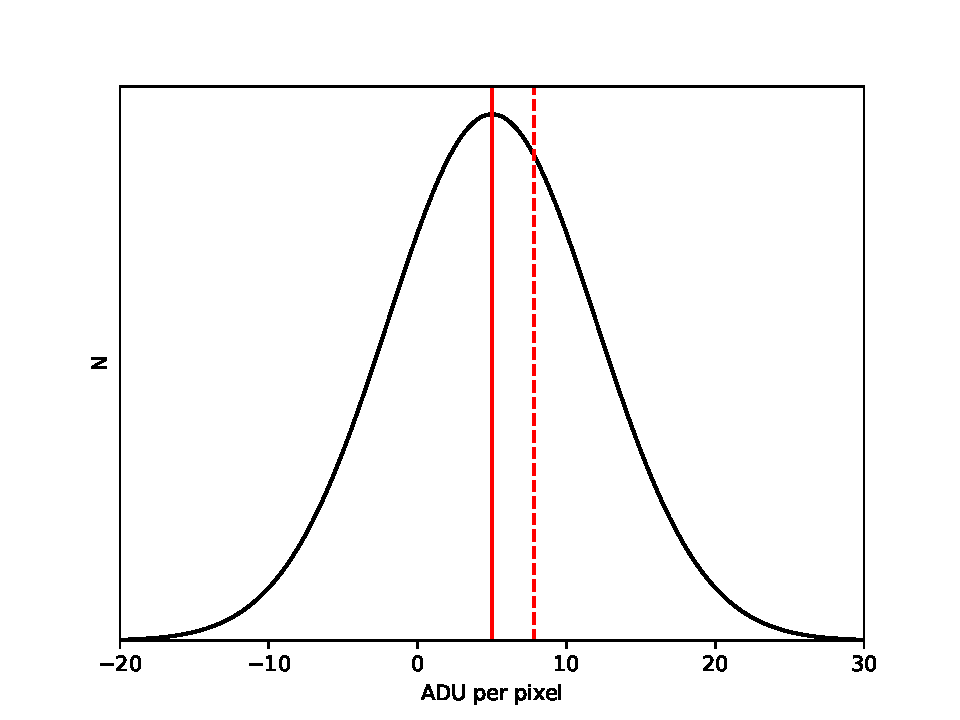
\includegraphics[width=0.7\textwidth]{figures/observations/bias_frame_histogram.pdf}
    \caption{Illustrating the effect of omitting negative values on the average of a distribution. The black line is a Gaussian distribution with an average of 5 and a standard deviation of 7. The vertical dashed line shows the `true' average of 5 ADU, and the vertical red line shows the average given by an ADC that reports negative electron counts as 0.}
    \label{fig:observations:bias frame histogram}
\end{figure}
The readout electronics of a CCD are not perfect, and contribute a small amount of gaussian noise to each pixel called readout noise. The ADC is only capable of recording {\it positive integer values}, and functionally discards negative pixel counts. To illustrate why this is an issue, take the exaggerated example of a readout noise of $7 e^-/{\rm px}$ on a region of the CCD that is stimulated by $5 e^-/{\rm px}$. If negative values are limited to 0, the effect is to increase the average, and Figure~\ref{fig:observations:bias frame histogram} illustrates the effect of discarding negative counts.
This will have a small corrupting effect on low-signal areas of the CCD, specifically the sky background which theoretically should be exactly zero.

To prevent this, a small bias voltage is applied to each pixel, raising the `floor' away from zero and preventing noise from giving negative readings. To then remove this bias voltage from observations, zero second exposures of a masked detector are taken to characterise the bias voltage for each pixel, and are subtracted off each subsequent exposure. These are known as bias frames, and are subtly altered by different instrument setups (i.e. binning pixels together when reading them out, or when only reading out partial images), so ideally a bias frame is taken for each different instrument setup.


\subsubsection{Flat fielding}

The response of each pixel to photons is similar, but is not equal. In addition, the optics of the telescope are not perfect (e.g. dust or other imperfections in lenses and mirrors) and throughput can vary across the field of view (vignetting). These effects mean that each exposure the instrument takes is multiplied by this response pattern.
In order to characterise this pattern, an exposure is taken of a known uniform brightness, for example a specialised light box with a high degree of uniformity. 
However, a simpler approach is to observe the sky during sunset, when the sky is still bright and the contribution of light from stars is largely negligible. 
The residual stellar light should still be removed, so to completely eliminate stars from the flat field observation, many exposures are taken and the telescope is nudged by a small amount every few seconds. Then, since the stars move between each exposure, calculating the median frame will effectively remove stars from the image, leaving behind only the pixel response pattern. 
Now, by dividing each exposure by the flat image, we can remove this pattern from future images. 


\subsubsection{Aperture photometry}

\todo{proofread}
While stars are theoretically point sources, we observe them through the atmosphere and the optics of the telescope, which acts to spread the light from a star, typically by 1-3 arcseconds. As such, to find the total flux of a star we must sum the contributions to flux from all pixels containing flux, and the HiPERCAM pipeline has two methods for this: `normal' extraction and `optimal' extraction.

Normal extraction is very simple. The user specifies one or more `reference' stars, and one or more `target' stars. The pixel ADU counts around the reference stars are plotted as a function of their radial distance to the peak flux, and the flux distribution is fitted with a Gaussian or Moffat profile. The Full-Width at Half Maximum (FWHM) of this distribution fit is calculated, and all pixels within $x \times \mathrm{FWHM}$ of the peak flux are simply summed to give the extracted flux of a source, cutting off some amount of the wings of the flux distribution. Here, $x$ is a user-defined parameter and while in theory a large value of $x$ would be desirable to capture all flux from a source, adding extra pixels contributes to the readout noise of the detection, and increasing $x$ results in diminishing returns due to the small amounts of flux contained in the wings.
Also, as the same fraction of light from each source should be lost from both the target sources and reference sources, cutting out these wings should not alter the flux ratio between the sources.

In many cases, it is preferable to use the `optimal' extraction method, described by \citet{naylor1998}. Here, a weight is taken into account when summing the flux contributions of each pixel based on the {\it expected} contribution to the overall flux. This can give an improvement of $\sim 10\%$ to the signal-to-noise ratio, especially in faint sources, as this approach is more robust against poor profile fits. Source profiles often diverge from the idealised Gaussian or Moffat profiles due to inconsistencies in seeing conditions or telescope guiding, and these effects are more pronounced in fainter sources. 

Finally, the sky is not perfectly black, due to the scattering effects of the atmosphere and telescope optics, and must be subtracted from the extracted flux of the sources. This is done by taking an annulus about each source, and assuming it is solely make up of sky background signal. The inner edge of the annulus is selected to be far enough from the source that none of the target's signal is present, and the outer edge is limited by contamination by other sources, and by very large annuli starting to become sensitive to sky variations across the image. The sky signal per pixel is then subtracted from each target pixel to isolate the target flux.




\section{Photometric calibration}
\label{sect:photometric extraction and calibration}

A comparison star in the same frame as the target was used to account for transparency variations, and standard stars from \citet{smith2002} were used to transform the lightcurves from ADU to the SDSS $u'g'r'i'z'$ photometric system. At the core of the photometric calibrations is the following expression of the apparent magnitude in some band, $m_{app}$, of a target,
\begin{equation}
    \label{eqn:observations:instrumental magnitude from scratch}
    m_{app} = m_{inst} + \chi k_{ext} + m_{zp} + C_{inst}c_{m}
\end{equation}
where $m_{inst}$ is the instrumental magnitude, $-2.5 \rm log(ADU)$, $\chi$ is the airmass of the obervation and $k_{ext}$ is the atmospheric extinction coefficient in the relevant band. $m_{zp}$ is the zero point offset of the instrument, calculated from photometric standard stars, ideally taken on the night of an observation. $c_{m}$ is the colour term correction between the response curve of the instrument, and the target photometric system, and $C_{inst}$ is a diagnostic instrumental colour. Each of these terms must be properly handled, and are discussed in turn. 


\subsection{Calculating atmospheric extinction coefficients}
\label{sect:calcualting atmospheric extinction}

Atmospheric extinction was calculated using the longest continuous observation available within a reasonable time from target observations.
The atmospheric extinction values are reported in Table~\ref{table:atmos_extinction}\todo{Currently, this is only for a very narrow range of the actual observations. Generalise this table to include all instruments and locations.}.

To calculate the atmospheric extinction coefficients, aperture photometery was extracted for five sources in these long observations, and the instrumental magnitude, $m_{\rm inst}$, vs airmass, $\chi$, was fit with a straight line for each source. 
The gradients of these lines are the atmospheric extinction coefficients, $k_{\rm ext}$, for the relevant band, and the y-intercept is the instrumental magnitude of that object above the atmosphere, $m_{\rm inst,0}$:
\begin{align*}
    m_{\rm inst} =& m_{\rm inst,0} + \chi k_{\rm ext} 
\end{align*}

\begin{table}
    \centering
    \caption{Atmospheric extinction coefficients for La Silla, derived from ULTRACAM/NTT observations.}
    \label{table:atmos_extinction}
    \begin{tabular}{cccc}
        \hline
        Date of Observation & Airmass Range & Band & $k_{ext}$ \\
        \hline
        \hline
        14 Oct 2018   & 1.30-1.98 & $u_{\rm reg}$ & $0.4476$ \\
                      &           & $g_{\rm reg}$ & $0.1776$ \\
                      &           & $r_{\rm reg}$ & $0.0861$ \\
        \hline
        30 Sept 2019  & 1.03-1.63 & $u_{\rm sup}$ & $0.4867$ \\
                      &           & $g_{\rm sup}$ & $0.1803$ \\
                      &           & $r_{\rm sup}$ & $0.0713$ \\
        \hline
    \end{tabular}
\end{table}


\subsection{Transformations between filter systems}
\label{sect:observations:colour correction method}

ULTRACAM and HiPERCAM use an SDSS-\emph{like} filter system with higher efficiency bandpasses, referred to as Super SDSS. There are three relevant photometric paths:
\begin{itemize}
\item SDSS filters, $u', g', r', i', z'$;
\item ULTRACAM/ULTRASPEC SDSS, $u_{\rm reg}, g_{\rm reg}, r_{\rm reg}, i_{\rm reg}, z_{\rm reg}$;
\item Super SDSS, $u_{\rm sup}, g_{\rm sup}, r_{\rm sup}, i_{\rm sup}, z_{\rm sup}$.
\end{itemize}

We aim to place our photometery in the SDSS $u'g'r'i'z'$ system, as this is the system later used by the white dwarf atmospheric models. The $u_{\rm reg}, g_{\rm reg}, r_{\rm reg}, i_{\rm reg}$\ filters were sufficiently similar to standard SDSS filters that the uncorrected magnitudes of standard reference stars from \citet{smith2002} could be used to calibrate absolute photometery without issue. However, with the new filters, there was concern that the different shape of the sensitivity curve, particularly in the $u'$\ band, differ enough from the standard filters to cause issues with our photometric calibration. Figure~\ref{fig:sdss vs super filters}\todo{Make a version of this for HiPERCAM and ULTRASPEC} illustrates the change in throughput between the SDSS photometric system, and the Super SDSS filters, on ULTRACAM on the NTT. 

\begin{figure}
    \centering
    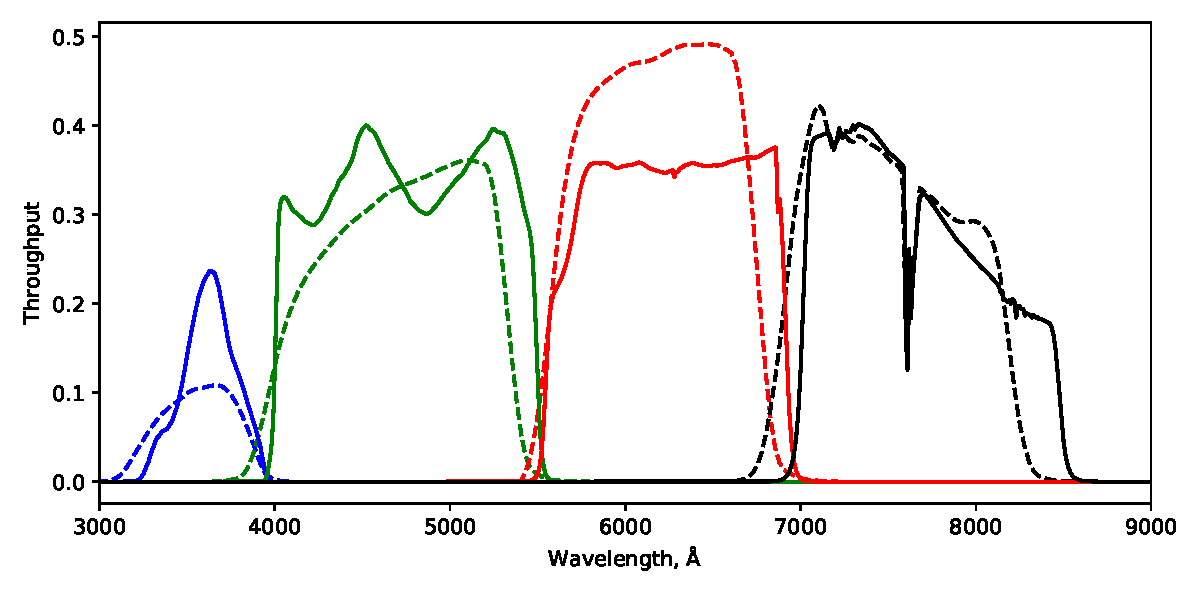
\includegraphics[width=\columnwidth]{figures/three_cvs_with_weird_colours/GeneralFigs/bandpass_diffs_SDSS_dots_UCAMNTT_solid.pdf}
    \caption{The differences in photometric throughput for SDSS filter system (dotted lines), and ULTRACAM Super SDSS filters, for ULTRACAM mounted on the NTT (solid lines). Blue: $u$ bands, Green: $g$ bands, Red: $r$ bands, Black: $i$ bands. Both throughputs include atmospheric extinction of $\chi = 1.3$.}
    \label{fig:sdss vs super filters}
\end{figure}

% As the difference in magnitude between photometric systems will be dependent on the shape of a stars spectrum, calculating the colour terms between the three systems is important.

To perform the colour corrections, the following equation for the magnitude of a star was used, using the $g'$\ band as an example:
\begin{equation}
    \label{eqn:gen magnitudes}
    g' = g_{\rm inst} + \chi k_{\rm ext} + g_{\rm zp} + c_{\rm g, sup}(g'-r') 
\end{equation}
where $g_{\rm zp}$\ is the zero point, $g_{\rm inst} = -2.5 \rm log(ADU/{\it t}_{\rm exp})$
for an exposure time of $t_{\rm exp}$, and $c_{\rm g, sup}$\ is the colour term correction gradient. 

The optical path of each system was simulated using the \texttt{pysynphot} package, with measured throughputs of all ULTRACAM\todo{Generalise} components in the optical path. Models from \citet{Dotter2016} and \citet{Choi2016} were used to generate the \teff\ and \logg\ values of an $8.5$\ Gyr isochrone for main sequence stars with masses from 0.1 to 3 $M_\odot$. These span from \logg $= 3.73 \to 5.17$, and $\rm{T_{eff}} = 2900K \to 10,300K$. The Phoenix model atmospheres \citep{allard2012} were used to generate model spectra of each mass, which was then folded through each optical path to calculate an AB magnitude. In addition, white dwarf models with \logg$=8.5$\ were similarly processed \citep{koester2010, tremblay2009}, to asses the impact of the different spectral shape on the resulting colour terms.

We synthesised the colour terms between the SDSS and ULTRACAM\todo{generalise} Super SDSS systems, e.g., $g'-g_{\rm sup}$, for each model atmosphere. These data were plotted against SDSS colours, i.e. $(u'-g')$, $(g'-r')$, $(g'-i')$, and a straight line was fit to the colour relationship. In the example case of $g'-g_{\rm sup}$, this would be
\begin{align*}
    g' &= g_{\rm sup} + g_{\rm zp} + c_{\rm g, sup}(g'-r') \\
    % g' - g_{\rm sup} &= g_{\rm zp} + c_{\rm g, sup}(g'-r')
\end{align*}
Note we ignore the effects of secondary extinction. 
These relationships are shown in Figure~\ref{fig:all colour corrections} for all four ULTRACAM\todo{generalise} filters used to observe these CVs, and Table~\ref{table:all colour corrections}\todo{Generalise} contains the coefficients of each colour term.
$(u'-g')$\ was used to correct $u$\ magnitudes, $(g'-r')$\ was used to correct $g$\ and $r$\ magnitudes, $(g'-i')$\ was used to correct the $i$\ band.
These colour corrections are not generally the same for main sequence stars and white dwarfs, though the colours of the white dwarfs presented in this work are all such that the discrepancy is on the order of a few percent, and is considered negligible.

\begin{table}
    \centering
    \caption{Colour term best fit lines from Figure~\ref{fig:all colour corrections}. The data are modelled by equations of the form $(u'-u_s) = \phi + c_u(u'-g')$, with $c_u$\ being the relevant colour gradient.}
    \label{table:all colour corrections}
    \begin{tabular}{cccc}
        Correction & Diagnostic &   y-intercept, $\phi$\   & Colour Gradient \\
        \hline
        \hline
          $(u'-u_s)$ &  $(u'-g')$   & 0.003 & 0.036 \\
                    &  $(g'-r')$   & 0.033 & 0.063 \\
                    &  $(g'-i')$   & 0.038 & 0.044 \\
        \hline
          $(g'-g_s)$ &  $(u'-g')$   & -0.001 & 0.014 \\
                    &  $(g'-r')$   & 0.010  & 0.027 \\
                    &  $(g'-i')$   & 0.012  & 0.018 \\
        \hline
          $(r'-r_s)$ &  $(u'-g')$   & -0.017 & 0.016 \\
                    &  $(g'-r')$   & -0.004 & 0.032 \\
                    &  $(g'-i')$   & -0.002 & 0.022 \\
        \hline
          $(i'-i_s)$ &  $(u'-g')$   & -0.031 & 0.020 \\
                    &  $(g'-r')$   & -0.015 & 0.040 \\
                    &  $(g'-i')$   & -0.012 & 0.028 \\
        \hline
        \hline
    \end{tabular}
\end{table}

\begin{figure*}
    \centering
    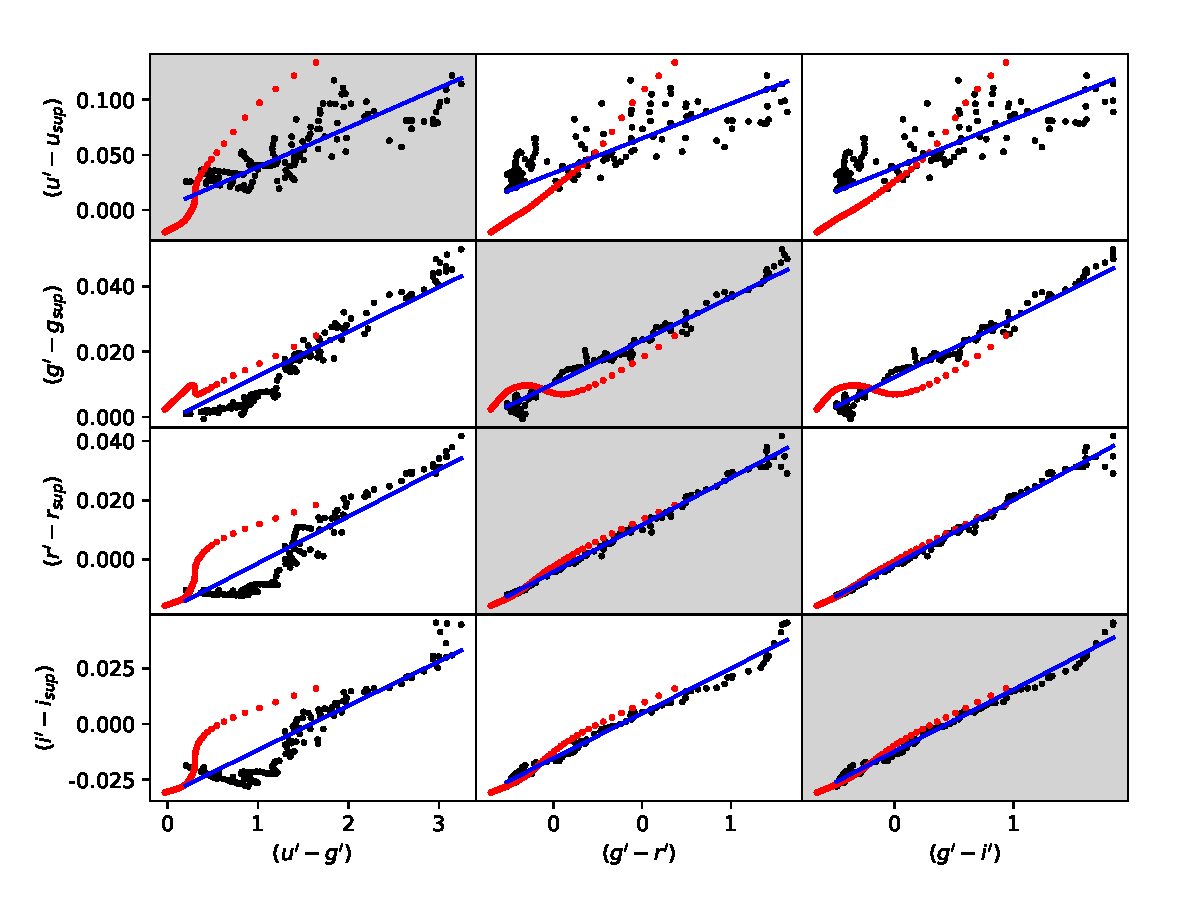
\includegraphics[width=0.9\textwidth]{figures/three_cvs_with_weird_colours/GeneralFigs/colour_term_tracks.pdf}
    \caption{The difference between the classic SDSS photometric system, and the ULTRACAM SuperSDSS filters on the NTT, as a function of SDSS colours, are calculated for model atmospheres. Red points are Koester white dwarf models, black points are Phoenix main sequence model atmospheres, and the blue line is the best fit straight line to both datasets. When applying colour corrections, the highlighted relations were used.}
    \label{fig:all colour corrections}
\end{figure*}

\subsection{Calculating comparison star magnitudes}
\label{sect:comparison star mag calc}

Equation \ref{eqn:gen magnitudes} was used to calculate the zero points in each band from the standard star, for the SDSS photometric system.
The comparison star SDSS magnitudes are then determined. As the colour term corrections are dependent on SDSS colours, an iterative approach was used to converge on these values. The SDSS magnitudes are related to the instrumental magnitudes by:
\begin{align*}
    u' =& u_{\rm inst,0} + u_{\rm zp} + c_{\rm u, sup}(u' - g') \\
    g' =& g_{\rm inst,0} + g_{\rm zp} + c_{\rm g, sup}(g' - r') \\
    r' =& r_{\rm inst,0} + r_{\rm zp} + c_{\rm r, sup}(g' - r')
\end{align*}
Initially, $u',g',r'$\ magnitudes are set equal to the instrumental magnitudes, and a new set of $u',g',r'$\ magnitudes are calculated. The new values are then used to repeat the calculation until a new iteration produces no change, typically after $\sim$4 loops. For the data taken with $u_{\rm sup},g_{\rm sup},i_{\rm sup}$\ filters, the process is identical but replaces $r$ with $i$.


\subsection{Producing a flux-calibrated target lightcurve}
\label{sect:flux calibrating the lightcurve}

Finally, the target lightcurves can be calculated. We need to both correct the target star lightcurve for transparency variations, and convert from counts to calibrated fluxes. As we are producing a flux-calibrated lightcurve in the SDSS photometric system using a significantly different photometric system, the simple ADU ratio between the target and comparison is insufficient. Consider the target star $g'$ magnitude and flux, $g^t, F^t$, and comparison star $g'$ magnitude and flux, $g^c, F^c$:
\begin{align*}
    g^t =& g^t_{\rm inst,0} + g_{\rm zp} + c_{\rm g, sup}(g'-r')^t \\
    g^c =& g^c_{\rm inst,0} + g_{\rm zp} + c_{\rm g, sup}(g'-r')^c \\
\end{align*}
since,
\begin{equation*}
    g^t - g^c = -2.5{\rm log}\Big(\frac{F^t}{F^c}\Big) \\
\end{equation*}
we can write
\begin{align*}
    % g^t - g^c =& g^t_{\rm inst,0} - g^c_{\rm inst,0} + c_{\rm g, sup}\big((g-r)^t - (g-r)^c\big) \\
    \frac{F^t}{F^c} =& 10^{-0.4(g^t_{\rm inst,0} - g^c_{\rm inst,0})} \cdot 10^{-0.4c_{\rm g, sup}\big((g'-r')^t - (g'-r')^c\big)} \\
    % \frac{F^t}{F^c} =& \frac{ADU^t/s}{ADU^c/s}\cdot 10^{c_{\rm g, sup}\big((g-r)^t - (g-r)^c\big)} \\
    \frac{F^t}{F^c} =& \frac{ADU^t}{ADU^c}\cdot K^{t,c} \\
\end{align*}
where $K^{t,c} = 10^{-0.4c_{\rm g, sup}\big((g'-r')^t - (g'-r')^c\big)}$.
This accounts for differences in wavelength response between the two systems when calculating the flux ratio, and is applied to each frame. The $(g'-r')^t$\ magnitudes are calculated using a sigma-clipped mean instrumental magnitudes computed from all frames in the observation. In practice, the factor $K^{t,c}$\ varies from $\sim 1.0 - 1.1$\ across the three systems. 

ASASSN-16kr was observed in both the standard SDSS filters in 2018, and the super SDSS filters in 2019. This presented an opportunity to compare the corrected 2019 data with the fluxes observed in 2018. Additionally, both ASASSN-16kr and SSSJ0522-3505 use multiple standard stars across observations, which should agree if the calibration has been done correctly. In all cases, the flux-calibrated lightcurves were similar and the white dwarf colours consistent, suggesting that this method of flux calibration is indeed accurate.

To account for residual error in flux calibration, we add a 3\% systematic error in quadrature to the white dwarf fluxes when fitting for the effective temperature.


\section{Catalogue of observations}

The observations analysed in this work span the full decade from 2011, through to 2021, and have been taken from multiple sites as the instruments move from telescope to telescope. To aid with the readability, a key is provided in Table~\ref{tab:observation acronyms} of the acronyms used for instruments and telescopes. 



\begin{table}
    \centering
    \begin{tabular}{c|c}
        Acronym & Expansion \\
        \hline
        NTT & New Technology Telescope \\
        GTC & Gran Telescopio Canarias \\
        TNT & Thai National Telescope \\
        WHT & William Herschel Telescope \\
        VLT & Very Large Telescope \\ 
        HCAM & HiPERCAM \\
        UCAM & ULTRACAM \\
        USPEC & ULTRASPEC \\
    \end{tabular}
    \caption{Acronyms used in the observation summaries.}
    \label{tab:observation acronyms}
\end{table}
